\chapter{动态规划}
如果一个问题具有以下两个要素:
\begindot
\item 最优子结构(optimal substructure)
\item 重叠子问题(overlap subproblem)
\myenddot
则可以用动态规划求最优解。

动态规划分为4个步骤:
\begindot
\item 描述最优解的结构。即抽象出一个状态来表示最优解。
\item 递归的定义最优解的值。找出状态转移方程,然后递归的定义
\item 计算最优解的值。典型的做法是自底向上,当然也可以自顶向下。
\item 根据计算过程中得到的信息,构造出最优解。如果我们只需要最优解的值,不需要最
优解本身,则可以忽略第4步。当执行第4步时,我们需要在第3步的过程中维护一些额外的
信息,以便我们能方便的构造出最优解。
\myenddot
在第1步中,我们需要抽象出一个“状态”,在第2步中,我们要找出“状态转移方程”,然后才能
递归的定义最优解的值。第3步和第4步就是写代码实现了。

写代码实现时有两种方式,“递归(recursive)+自顶向下(top-down)+表格(memoization)”和
“自底向上(bottom-up)+表格”。

动规用表格将各个子问题的最优解存起来,避免重复计算,是一种空间换时间。

动规与贪心的相同点:最优子结构。

不同点:1、动规的子问题是重叠的,而贪心的子问题是不重叠的(disjoint subproblems);
2、动规不具有贪心选择性质。

分治和贪心的相同点:disjoint subproblems。

\section{数字三角形} %%%%%%%%%%%%%%%%%%%%%%%%%%%%%
有一个由非负整数组成的三角形,第一行只有一个数,除了最下一行之外每个数的左下角和右下
角各有一个数,如图~~\ref{fig:numbersTriangle}所示。

\begin{center}
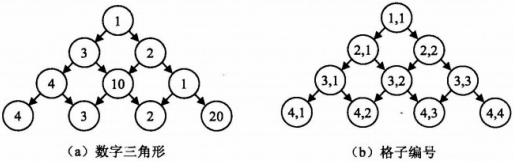
\includegraphics[width=360pt]{numbers-triangle.png}\\
\figcaption{数字三角形问题}\label{fig:numbersTriangle}
\end{center}

从第一行的数开始,每次可以往左下或右下走一格,直到走到最下行,把沿途经过的数全部加起来。
如何走才能使得这个和最大?

\textbf{Input}

Your program is to read from standard input. The first line contains one integer N: the 
number of rows in the triangle. The following N lines describe the data of the triangle. 
The number of rows in the triangle is > 1 but <= 100. The numbers in the triangle, 
all integers, are between 0 and 99.

\textbf{Output}

Your program is to write to standard output. The highest sum is written as an integer.

\textbf{Sample Input} \\
5 \\
7 \\
3 8 \\
8 1 0  \\
2 7 4 4 \\
4 5 2 6 5

\textbf{Sample Output} \\
30

\subsubsection{分析}
这是一个动态决策问题,在每层有两种选择,左下或右下,因此一个n层的数字三角形有$2^n$条路线。

可以用回溯法,用回溯法求出所有可能的路线,就可以从中选出最优路线。但是由于有$2^n$条路线,
回溯法很慢。

本题可以用动态规划来求解(具有最有子结构和重叠子问题两个要素,后面会看到)。把当前位置(i,j)看
成一个状态,然后定义状态(i,j)的指数函数d(i,j)为从位置(i,j)出发时能得到的最大和(包括格子(i,j)本
身的值a(i,j))。在这个状态定义下,原问题的解是d(1,1)。

下面来看看不同状态之间是怎样转移的。从位置(i,j)出发有两种决策,如果往左走,则走到(i+1,j)后需要求
“从(i+1,j)出发后能得到的最大和”这一子问题,即d(i+1,j),类似地,往右走之后需要求d(i+1,j+1)。应该
选择d(i+1,j)和d(i+1,j+1)中较大的一个,因此可以得到如下的状态转移方程:
$$d(i,j)=a(i,j)+\max{d(i+1,j), d(i+1,j+1)}$$

\subsubsection{代码}
版本1,自顶向下。

\begin{Codex}[label=numbers_triangle1.c]
#include<stdio.h>
#include<string.h>

#define MAXN 100

int n, a[MAXN][MAXN], d[MAXN][MAXN];

static int max(const int x, const int y) {
    return x > y ? x : y;
}

/**
 * @brief 求从位置(i,j)出发时能得到的最大和
 * @param[in] i 行
 * @param[in] j 列
 * @return 最大和
 */
static int f(const int i, const int j) {
    if(d[i][j] >= 0) {
        return d[i][j];
    } else {
        return d[i][j] = a[i][j] + (i == n-1 ? 0 : max(f(i+1, j+1), f(i+1, j)));
    }
}

int main() {
    int i, j;
    memset(d, -1, sizeof(d));

    scanf("%d", &n);
    for(i = 0; i < n; i++)
      for (j = 0; j <= i; j++) scanf("%d", &a[i][j]);
    
    printf("%d\n", f(0, 0));
    return 0;
}

\end{Codex}

版本2,自底向上。

\begin{Codex}[label=numbers_triangle2.c]
#include<stdio.h>
#include<string.h>

#define MAXN 100

int n, a[MAXN][MAXN], d[MAXN][MAXN];

static int max(const int x, const int y) {
    return x > y ? x : y;
}

/**
 * @brief 自底向上计算所有子问题的最优解
 * @return 无
 */
static void f() {
    int i, j;
    for (i = 0; i < n; ++i) {
        d[n-1][i] = a[n-1][i];
    }
    for (i = n-2; i >= 0; --i)
      for (j = 0; j <= i; ++j)
        d[i][j] = a[i][j] + max(d[i+1][j], d[i+1][j+1]);
}

int main() {
    int i, j;
    memset(d, -1, sizeof(d));

    scanf("%d", &n);
    for(i = 0; i < n; i++)
      for (j = 0; j <= i; j++) 
          scanf("%d", &a[i][j]);

    f();
    
    printf("%d\n", d[0][0]);
    return 0;
}
\end{Codex}

\subsubsection{类似的题目}
与本题相同的题目:
\begindot
\item 《算法竞赛入门经典》\footnote{刘汝佳,算法竞赛入门经典,清华大学出版社,2009}第159页9.1.1节
\item  POJ 1163 - The Triangle, \myurl{http://poj.org/problem?id=1163}
\myenddot

与本题相似的题目:
\begindot
\item  TODO
\myenddot

\section{最长公共子序列} %%%%%%%%%%%%%%%%%%%%%%%%%%%%%%

\section{0-1背包} %%%%%%%%%%%%%%%%%%%%%%%%%%%%%%